\chapter{Introduction}\label{ch:introduction}

Electronic voting represents one of the most challenging applications of modern cryptography: a system must simultaneously prove that a voter is eligible (accountability) while ensuring that no one---not even the system operators---can determine how that voter voted (privacy). This chapter establishes the context, formally defines the problem, and outlines our approach.

\section{Background}

\subsection{The Democratic Election Challenge in Sri Lanka}

Sri Lanka is a parliamentary democracy with a complex multi-tier electoral structure. National elections are conducted across 22 electoral districts containing 160 polling divisions, administered through approximately 14,000 Grama Niladhari (Village Officer) divisions, serving over 16 million registered voters.

The current paper-ballot system faces significant challenges: counting delays of 24--48 hours, high logistical costs, susceptibility to human error, limited accessibility for disabled or overseas citizens, and expensive recounting processes.

\begin{figure}[H]
\centering
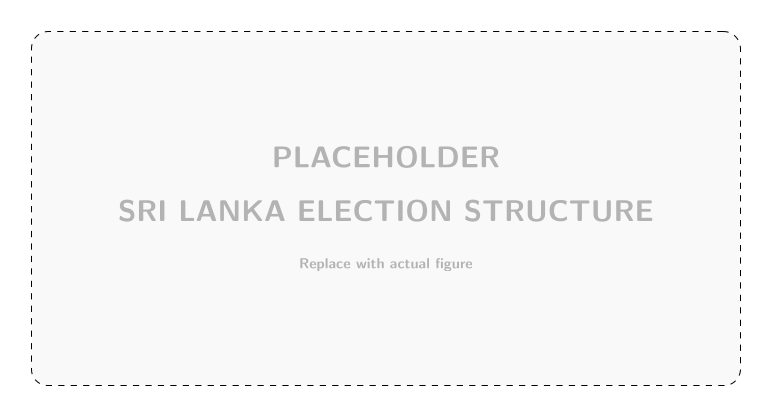
\includegraphics[width=0.85\textwidth]{Images/fig_sri_lanka_election_structure.png}
\caption{Sri Lanka's electoral hierarchy from the Election Commission down to 16+ million individual voters.}
\label{fig:sl-structure}
\end{figure}

\subsection{Formal Requirements for Secure Electronic Voting}

Any electronic voting system must satisfy four fundamental properties:

\begin{definition}[Eligibility Verification]
Only citizens on the certified register may vote; each may cast at most one ballot.
\end{definition}

\begin{definition}[Ballot Privacy]
No entity can determine how any specific voter cast their ballot.
\end{definition}

\begin{definition}[End-to-End Verifiability]
Any participant can verify that their ballot was recorded correctly and that the tally is correct.
\end{definition}

\begin{definition}[Coercion Resistance]
A voter cannot produce evidence proving how they voted to a third party.
\end{definition}

\subsection{Why Blockchain Alone Is Insufficient}

Blockchain provides integrity and transparency, but standard transactions reveal the sender address. On Ethereum, a vote transaction exposes: \texttt{From: 0xAlice To: Voting.sol Data: vote(3)}. If the address is linked to Alice's identity, ballot privacy is destroyed. Prior blockchain voting systems suffered this exact vulnerability.

\subsection{Zero-Knowledge Proofs: The Key Enabler}

Zero-knowledge proofs resolve the eligibility--privacy tension. Instead of revealing identity, a voter proves: \textit{``I am SOME valid registered voter''} without revealing which one. Combined with an ephemeral wallet for submission, this achieves cryptographic unlinkability between voter and ballot.

\begin{figure}[H]
\centering
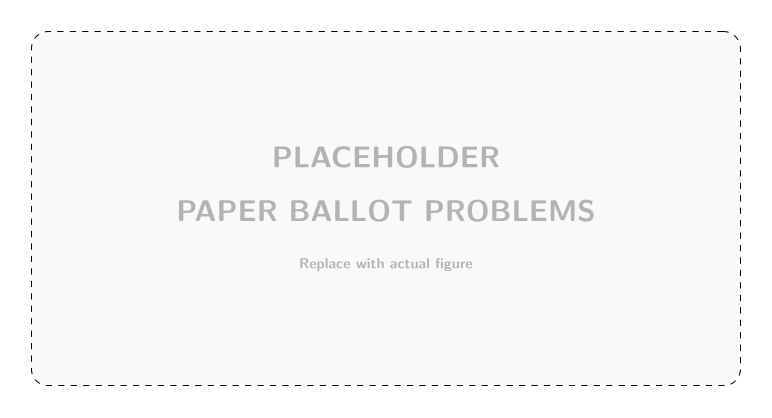
\includegraphics[width=0.85\textwidth]{Images/fig_paper_ballot_problems.png}
\caption{Paper ballot challenges and how our ZK-based system addresses each.}
\label{fig:paper-problems}
\end{figure}

\section{Problem Statement}

\begin{enumerate}
    \item \textbf{Ballot--voter linkability}: Blockchain transaction senders reveal voter identity.
    \item \textbf{Centralized trust}: Systems like Helios/MACI require trusted intermediaries.
    \item \textbf{Administrative infidelity}: Prototypes ignore real government structures.
    \item \textbf{Economic barriers}: Gas fees exclude voters from participation.
    \item \textbf{Weak authentication}: Wallet-only auth provides no physical presence verification.
    \item \textbf{Sybil vulnerability}: No national-level identity de-duplication.
\end{enumerate}

\section{Objectives and Scope}

\subsection{Objectives}
\begin{enumerate}
    \item Design a ZK circuit proving voter membership without revealing identity.
    \item Develop smart contracts with five layers of on-chain fraud prevention.
    \item Build a custom gasless blockchain embedding the EVM.
    \item Develop a mobile app with hardware security and on-device proof generation.
    \item Implement web administration for Election Authority and GN officers.
    \item Model Sri Lanka's 160-division structure with on-chain national aggregation.
    \item Achieve formal voter--ballot unlinkability:
\end{enumerate}

\begin{equation}
\Pr\left[\mathcal{A}(\text{chain}) \to (\text{Voter}, \text{Ballot})\right] \le \frac{1}{|\mathcal{V}|} + \text{negl}(\lambda)
\label{eq:anon-intro}
\end{equation}

\subsection{Scope}
\textbf{In scope}: Complete voting pipeline, Android mobile app, web console, custom blockchain, 54-test suite, performance evaluation.

\textbf{Out of scope}: Full ballot secrecy (homomorphic tallying), formal verification (Lean 4), production deployment, iOS testing.

\section{Methodology Overview}

The project followed an iterative bottom-up methodology:
\begin{itemize}
    \item \textbf{Phase 1 (Nov 2025 -- Feb 2026)}: ZK circuit, smart contracts, proof system, test suite, web frontend.
    \item \textbf{Phase 2 (Mar -- Jul 2026)}: Custom blockchain, mobile app, three-factor auth, multi-division, integration.
\end{itemize}

\section{Team Contributions}

\begin{table}[H]
\centering
\caption{Team Member Responsibilities}
\label{tab:team}
\begin{tabular}{|l|l|p{6cm}|}
\hline
\textbf{Member} & \textbf{Reg. No.} & \textbf{Primary Responsibilities} \\
\hline
K.K.R. Kumarasinghe & EG/2021/4632 & Smart contracts, testing, deployment \\
\hline
R.M.D. Madhusankha & EG/2021/4655 & Custom Go blockchain, REST API \\
\hline
R.M.T. Pradeepani & EG/2021/4725 & ZK circuit, cryptographic design \\
\hline
K.K.M.P. Ranasinghe & EG/2021/4735 & Mobile app, web frontend, auth \\
\hline
\end{tabular}
\end{table}

\begin{figure}[H]
\centering
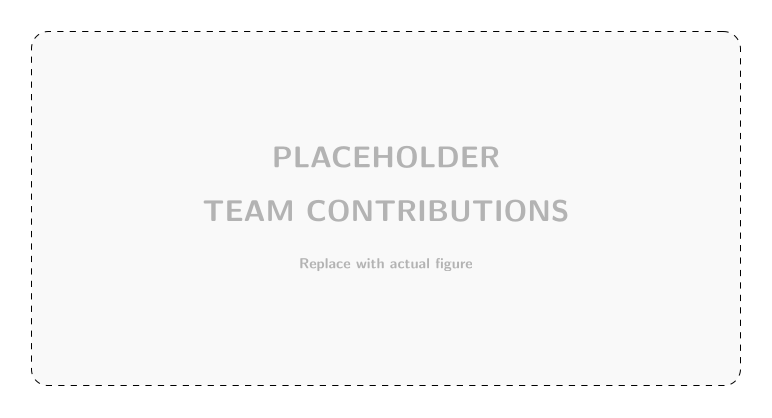
\includegraphics[width=0.75\textwidth]{Images/fig_team_contributions.png}
\caption{Team member contribution areas and overlap in integration work.}
\label{fig:team-contributions}
\end{figure}

\section{Report Organization}

The report is organized into 9 chapters covering the complete project from literature through implementation to evaluation.
